\chapter[SPARCC: An R package for estimating power to detect QTL through simulated experiments in the realized Collaborative Cross]{SPARCC: An R package for estimating power to detect QTL through simulated experiments in the realized Collaborative Cross
\footnote{This chapter represents a mature draft of a manuscript currently in preparation, with slight modifications made for the format. Current author line and title are: Keele GR\textsuperscript{*}, Crouse WL\textsuperscript{*}, Kelada SNP, Valdar W. SPARCC: An R package for calculating power through simulation of QTL mapping experiments in the realized Collaborative Cross. Co-first authors\textsuperscript{*}.}}
\label{chap:sparcc}

\section{Introduction}

The Collaborative Cross (CC) is a panel of multiparental (MPP) recombinant inbred (RI) strains of laboratory mouse, descended from eight inbred founder strains \citep{Threadgill2002,Churchill2004}. These founders represent three subspecies of the domesticated house mouse \textit{Mus musculus} \citep{Yang2011}, imbuing the CC panel with far greater genetic variation than traditional inbred strains, in particular, the presence of alleles inherited from wild-derived strains. The CC panel is a powerful tool that provides a genetically diverse set of reproducible genomes \citep{Hall2012,Srivastava2017}. 

The genetic diversity present within the CC makes it ideal for modern genetic studies of genetically diverse populations, such as for modeling complex disease in humans. Drawing from the presence of unique allelic combinations across the genomes, the CC can often provide better models of human disease, usually not possible in traditional inbred mouse strains \citep{Rogala2014,Gralinski2015}. The CC are also valuable for joint analyses with its outbred sister population, the Diversity Outbred (DO) stock \citep{Churchill2012,Chick2016}. Finally, the genetic diversity can be interrogated through quantitative trait loci (QTL) mapping \citep{Aylor2011,Kelada2016,Donoghue2017,Maurizio2017}, including the ability to map phenotypes that can only be measured from counter-factual observations, such as drug response, due to its genetic reproducibility \citep{Mosedale2017}. 

At the time of this writing, 72 CC strains were available, falling well below the initial stated goal of 1000 RI strains. The reduced number of strains is due to extinctions during the inbreeding phase, likely because of allelic incompatibilities across subspecies \citep{Shorter2017}. Although these extinctions have provided an unexpected source of insight into the genetics of fertility-related traits, it is unclear to what extent the reduction in CC strains reduces the power to map QTL. Initial power estimates were based on many simulated CC genomes \citep{Valdar2006a}; however, these calculations do not reflect the number of available strains or the actual founder mosaics realized in the genomes of the currently available strains. 

Power dynamics have been investigated in genome-wide association studies (GWAS) in humans \citep{Purcell2003,Klein2007}, though they do not assess important experimental design considerations for reproducible experimental populations like the CC, for which the same genomes are used across many studies, and possibly include replicate observations. \cite{Kaeppler1997} performed power calculations in RI strains analytically, though these estimates will not reflect the specific genomes of the CC, nor the specific statistical procedures used to map in the CC. \cite{Falke2011} and \cite{Takuno2012} do use simulations to estimate QTL mapping in RI panels and near-isogenic lines (NIL), but their focus is more within the context of plant RI panels, resulting in simulations that reflect those model systems more than those of animal models. This supports the need to explore QTL mapping power in the realized CC.

Our R package, Simulated Power Analysis of the Realized Collaborative Cross (SPARCC), is a tool that evaluates power to map QTL by performing efficient regression-based association analysis of simulated QTL using the currently-available CC genomes. SPARCC is highly flexible, allowing researchers to tailor their calculations based on the CC strains available to them and the genetic architecture of their phenotypes.

\section{Methods}

\subsection{Data simulation}

SPARCC allows the user to simulate CC phenotypes that reflect a range of underlying genetic architectures. These are controlled by various input parameters to the \texttt{sim.CC.data()} function which we will describe in detail. The data-generating model is:
\begin{equation}
	\by = \bone\mu + \underbrace{\bZ\bX\bbeta}_{\text{QTL effect}} + \underbrace{\bZ\bdelta}_{\text{Strain effect}} + \underbrace{\bepsilon}_{\text{Noise effect}},
    \label{eq:general_sim}
\end{equation}
where $\by$ is the phenotype, $\mu$ is the intercept, $\bZ$ is the strain design matrix, $\bX$ is the QTL allele dosage matrix, $\bbeta$ is the QTL effect vector, $\bdelta$ is the background strain effect, and $\bepsilon$ is an unstructured, random error term. We will describe each component of Eq \ref{eq:general_sim} in greater detail, with additional options for \texttt{sim.CC.data()} described in \textbf{Simulation Documentation}.

\subsubsection{QTL effect}
The QTL effect represents the component of the phenotype that is determined by the founder haplotype states at a locus. By default, this locus is sampled from the genome, but it can also be user-specified. The QTL effect in Eq \ref{eq:general_sim} is simplified relative to the actual simulation procedure, which specifies a number of functional alleles and the assignment of founders haplotypes to these alleles \citep{Yalcin2005} through 
\begin{equation}
	\bX = \bD\bA\bM,
    \label{eq:sdp}
\end{equation}
where $\bD$ is the matrix of haplotype pairs, also referred to as diplotypes, at the QTL, $\bA$ is an additive model matrix that maps diplotypes to haplotype dosages, and $\bM$ is a founder-to-allele mapping matrix. Though the haplotype is described in terms of eight "alleles" corresponding to the founder haplotypes, it may be expected that the QTL effect results from fewer functionally distinct alleles than the number of founders, for example, via an underlying bi-allelic single nucleotide polymorphism (SNP). Thus, the matrix $\bM$ encodes a mapping between the founder haplotypes and a specified number of functional alleles, termed the allelic series. The allelic series can be randomly sampled within SPARCC or specified by the user. Assumptions about the allelic series may have a substantial influence on power, as some allelic configurations may be highly imbalanced or poorly-represented by the founder haplotypes at the QTL locus. 

The allelic series, the functional allele effect vector $\bbeta$, and the particular population will together determine the proportion of the phenotypic variance that the QTL controls, which we refer to as the QTL effect size. It follows that CC data can be simulated with respect to the QTL effect size in differing populations, for example the mapping population itself, with resulting powers highly specific to a given sample of CC strains. Alternatively, the CC data could be simulated with respect to a theoretical, more natural population that possesses the genetic variants present in the founder strains, which would represent the power to map variants segregating in the initial founders. We will present results from both approaches to simulating data based on QTL effect size.  

The function for simulating CC data is \texttt{sim.CC.data()}, which has a number of arguments that control the various components of this effect, which are described in detail in \textbf{Simulation Documentation}. The primary components of interest that can be controlled have been described, such as the QTL effect size, the allelic series ($\bM$), the set of CC strains, and the locus from which to simulate. The current version of SPARCC assumes a single QTL, though the procedure could be generalized to multiple QTL with few modifications. 

\subsubsection{Strain effect}

The background strain effect represents the aggregate genetic effect present in each strain, not including the simulated QTL. Many complex traits, such as height in humans \citep{Wood2014}, have highly polygenic and complex genetic architectures \citep{Phillippi2014}. It is possible, even expected, that any given QTL will have an individually small effect, despite the phenotype being highly heritable.

The phenotypic variability that results from strain background presents as additional noise with respect to identifying QTL. This is particularly clear in the the situation in which only a single observation of each strain is observed, at which point, $\bZ \rightarrow \bI$ in Eq \ref{eq:general_sim}, and $\bdelta$ and $\bepsilon$ are indistinguishable from each other. Replicate observations, an important feature of the CC, allow for the unstructured, individual error ($\bepsilon$) to be reduced, potentially improving the power to detect QTL. However, replicate observations will not reduce variability due to the background strain effect, and thus will not improve QTL mapping power in phenotypes with a large background strain effect. The options for \texttt{sim.CC.data()} that control the strain.effect are described in \textbf{Simulation Documentation}.

\subsubsection{Noise effect} 

The noise effect, or variation due to random error, will automatically be calculated as $$1 - \text{QTL effect} - \text{Strain effect},$$ which is used as the value of $\sigmasq$ for sampling $\bepsilon \sim \text{N}(\bzero, \bI\sigmasq)$. The error variance must be greater than zero.

\subsubsection{Robust power estimation}

Our intention is that SPARCC will serve as a flexible tool for calculating power in many different experimental and genetic contexts. The output of the CC data simulation is a matrix of outcomes, with each column $\bys$, the $s$\textsuperscript{th} simulation from equation \ref{eq:general_sim}. By default, we vary the set of CC strains, loci, and allelic series, producing power estimates that take into account many sources of uncertainty, and are thus broadly interpretable. Alternatively, an investigator may be interested in a more focused power calculation, for instance, on a set of CC strains that have already been chosen. Similarly, it could be used to estimate power for specific loci and allelic series configurations.

\subsection{Mapping procedure}

QTL mapping or genome-wide association involves testing the association of a phenotype with the genetic information at positions across the genome, often through a linear model. In mapping populations with well-characterized haplotypes, which can be probabilistically inferred \citep{Lander1987,Mott2000,Liu2010,Fu2012,Gatti2014,Zheng2015}, rather than association on typed variants, such as SNPs, the association between phenotype and haplotype is possible, a procedure called interval mapping \citep{Lander1989}, which formally takes into account the uncertainty in haplotype, requiring a computationally costly expectation-maximization (EM) procedure \citep{Dempster1977}. An approximation to interval mapping was proposed by \cite{Haley1992,Martinez1992} that uses standard linear regression (HK regression), which is computationally efficient, generally stable, and accurate when the information content on diplotype probabilities is high.

\subsubsection{Regression model}

The DEFAULT for SPARCC is to use HK regression on strain means across replicates \citep{Zou2006}. Thus, we fit each simulated phenotype $\bys$ using the following model:
\begin{equation}
	\bbarys = \bone\mu + \bP\bA\bbeta + \baltepsilon
    \label{eq:mapping_model}
\end{equation}
where $\bbarys$ is the vector of strain means, and $\baltepsilon$ is the residual on the means, which is expected to be distributed following $\baltepsilon \sim \text{N}(\bzero, \bI(\tausq + \frac{\sigmasq}{r}))$. The allelic series, encoded in $\bM$, is fixed to the eight allele model \citep{Gatti2014}. We note that this could lead to lower power when there are fewer functional alleles, particularly at loci in which the functional alleles are not well represented.

We compare the model fit of Eq \ref{eq:mapping_model} to the fit of a null model with just the intercept and obtain a p-value based on an F-test from the residual sums of squares (RSS) for the two models. Alternatively, the likelihood ratio test could be used, although the F-test is preferable given the relatively low number of CC strains. This procedure is performed for all loci, resulting in a genome scan for $\bys$. Power to map the simulated QTL is the proportion of $\bys$ for which the QTL was detected at a genome-wide significance threshold.

\subsubsection{Significance thresholds and power}

The CC panel is a balanced population with respect to founder genomic contributions, with limited levels of population structure, which supports the assumption of exchangeability. As such, we use permutations of $\bys$ to assess genome-wide significance based on controlling the family-wide error rate (FWER) \citep{Doerge1996}. Briefly, we sample $p$ permutations, which can be represented as $\bU_{p}\bys$, where $\bU$ is a permutation matrix that re-orders $\bys$ accordingly. We select the maximum $-\log_{10}\text{p-value}$ ($\logp^{(s)}_{p}$) from each $p$ genome scan of simulation $s$, which are used to fit an extreme value distribution (EVD) \citep{Dudbridge2004,Valdar2006c}, which represents a FWER-controlled null distribution from which to draw a significance threshold $\thresh$ for genome-wide FWER false positive probability $\alpha$. The QTL is mapped if the $\logp^{(s)} \ge \thresh$. Power, the probability that the simulated QTL is mapped follows:
\begin{equation}
	\text{Power} = \frac{\sum_{s=1}^{S} 1_{\logp^{(s)} \ge \thresh}}{S}
    \label{eq:power}
\end{equation}
where $1_{A}$ is the indicator function on whether $A: \logp^{(s)} \ge \thresh$ is satisfied. The power estimate in Eq \ref{eq:power} is a point estimate specific to the simulation procedure. Investigators should consider ranges of simulation settings, in particular varying the QTL effect size, number of strains, and number of replicates. Running SPARCC for multiple settings can then be used to produce useful power curves or tables.

\subsubsection{QR decomposition for fast regression}

Because the genome-wide scans SPARCC performs on simulated data from the realized CC genomes require permutations for determination of statistical significance, the underlying regression functionality must be highly optimized. We accomplish this through the QR matrix decomposition, which we will describe briefly \citep{Venables2002}. 

Let $\bX=\bP\bA$ be the $n \times m$ design matrix included in Eq \ref{eq:mapping_model}, with $m=8$ for SPARCC. The solution for $\bbeta$ from the least squares normal equations is $\widehat{\bbeta} = (\bX^{\text{T}}\bX)^{-1}\bX^{\text{T}}\by$. Through the QR decomposition, $\bX = \bQ\bR$, for which $\bQ$ is an $n \times p$ orthonormal matrix  ($\bQ^{\text{T}}\bQ = \bI)$ and $\bR$ is a $m \times m$ upper triangular matrix. With matrix algebra, it is fairly straightforward to show that $\widehat{\bbeta} = \bR^{-1}\bQ^{\text{T}}\by$, which is also more numerically stable than calculating $\widehat{\bbeta}$ through $(\bX^{\text{T}}\bX)^{-1}$. After solving for $\widehat{\bbeta}$, the RSS, and ultimately \logp, can be rapidly calculated. Because the SPARCC uses a simulation approach that involves regressing many permuted outcomes ($\bU_{p}\by^{(s)}$) on the same design matrices, computational efficiency can be vastly increased by pre-computing and saving the QR decompositions for all $\bX$.

Once the QR decomposition has been stored for a design matrix $\bX_{j}$, $j$ indexing locus, it is highly computationally efficient to conduct additional tests for any $\by$, thus encompassing all permuted outcomes $\bU_{p}\by$. If $\bX_{j}$ is the same across $S$ simulations, the boost in computation can extend beyond permutations to samples of $\bys$, as is the case when the set of CC strains is fixed. In effect, two cases result for SPARCC: when the set of CC strains is fixed, and when the set varies.
\begin{itemize}
	\item Fixed set of CC strains
    \begin{enumerate}
    	\item Store QR decompositions of $\bX_{j}$ for $j=1, 2, \ldots, J$
        \item Run genome scans for $\bys$ and $\bU_{p}\bys$ for $s=1, 2, \ldots, S \times p=1, 2, \ldots, P$
    \end{enumerate}
    \item Varied set of CC strains
    \begin{enumerate}
    	\item Store QR decompositions of $\bX_{js}$ for $j=1, 2, \ldots, J$
        \item Run genome scans for $\bys$ and $\bU_{p}\bys$ for $p=1, 2, \ldots, P$
        \item Repeat steps 1 and 2 for $s=1, 2, \ldots, S$
    \end{enumerate}
\end{itemize}
Varying the sets of CC strains increases computation time linearly with respect to $S$. If the investigators do not have a predefined set of strains, it is appropriate that this source of variability be incorporated into the power calculation.


\subsubsection{Performing genome scans}

The SPARCC function for running genome scans from the simulated data is \texttt{run.sim.scans()}, The primary argument is \texttt{sim.data}, which expects simulated data output from \texttt{sim.CC.data()}. There are additional arguments to restrict the scans to a subset of the chromosomes, to a subset of the simulated phenotypes, or to a subset of loci. Finally, the user can provide the precomputed QR decompositions and specify whether the output should return those decompositions, which can be expensive in terms of memory.

\subsection{Availability of data and software}

\subsubsection{R package} 

All analyses were conducted in the statistical programming language R \citep{RSoftware2018}. SPARCC is available as an R package on GitHub at \url{https://github.com/gkeele/sparcc}. SPARCC also depends upon QTL mapping functionality present in the R package miqtl, which is also available on GitHub at \url{https://github.com/gkeele/miqtl}.

\subsubsection{CC haplotype pair probabilities}

Founder haplotype probabilities for each CC strain are available on the CC resource website (\url{http://csbio.unc.edu/CCstatus/index.py?run=FounderProbs}). The diplotype probabilities were constructed using a hidden Markov model (HMM) for haplotype inference as previously described \citep{Liu2010}. The probabilities are based on genotype calls from the MegaMUGA SNP array that contains 77,800 genotype markers. We use probabilities corresponding to build 37 of the mouse genome, though build 38 is also available at the previously mentioned website.

\subsubsection{Haplotype data reduction}

We reduce the size of the CC haplotype probability data by averaging adjacent intervals that are similar in probabilities, in order to reduce the computational expense of scans. Adjacent sites were averaged if the maximum L2 norm between the probability vectors of all individual is less than 10\% of the maximum possible L2 norm ($\sqrt{2}$), ultimately reducing the cumulative storage from 610 MB to 288 MB. We store these data in a directory with a structure with which SPARCC is designed to interact. These data are available on GitHub at \url{https://github.com/gkeele/sparcc_cache}.

\section{Results and Discussion}

\subsection{Simple SPARCC example}

We provide a simple demonstration of simulating a data set, performing genome scans, determining thresholds of significance, and ultimately QTL mapping power. This example is computationally efficient because CC strains are not varied across simulations, though the locus is. We also provide run-time estimates for the main steps.

\begin{verbatim}
###############################################
### Useful functions for parsing haplotype data
> library(miqtl) 
> h <- DiploprobReader$new("./sparcc_cache/")
> set.seed(10)

### Grabbing random sample of 65 CC strains
> these.cc.lines <- sample(h$getSubjects(), size=65) 

> library(sparcc)
### Simulate 5 data sets:
#### Specified 65 CC strains
#### 5 replicate observations of each
#### 2 functional alleles, allelic series not specified
#### QTL effect size of 30%
#### Background Strain effect of 10%
> simple.data <- sim.CC.data(genomecache="./sparcc_cache/", 
                           	 CC.lines=these.cc.lines,
                             num.replicates=5,
                             num.sim=5,
                             num.alleles=2,
                             qtl.effect.size=0.3, 
                             strain.effect.size=0.1)

### Genome scans
> simple.scans <- run.sim.scans(sim.data=simple.data,
                                return.all.sim.qr=TRUE)

### Generating permutation index
> perm.index <- generate.perm.matrix(num.lines=65, 
                                     num.perm=100)

### Permutation scans
> thresh.scans <- run.perm.scans(perm.matrix=perm.index, 
                                 sim.CC.object=simple.data, 
                                 sim.CC.scans=simple.scans)

### Calculating significance thresholds
> all.thresh <- get.thresholds(thresh.scans=thresh.scans)

### Power estimate
> pull.power(sim.scans=simple.scans, 
			 thresh=all.thresh)
[1] 0.8

### Plot a genome scan of a single simulated phenotype
> single.sim.plot(simple.scans, 
                  thresh=all.thresh, 
                  phenotype.index=1)
###############################################
\end{verbatim}

Plots of the simulated CC genome scans produced by the above code are in \textbf{Figure \ref{fig:example_scans}}.

\subsubsection{Run-time performance}

The simple example was run locally on an Early 2015 MacBook Pro with a 2.9 GHz Intel Core i5 processor and 8 GB of RAM. The data simulation and genome-wide scans for five phenotypes took 32.3781 seconds. Computational time increases linearly with number of phenotypes simulated. Computational times will also decrease for lower numbers of CC strains. 100 permutations for 5 simulated phenotypes took 9.315485 minutes. Although the time expense for SPARCC is not trivial, the overall process is highly optimized; this simple example involves fitting 5 phenotypes $\times$ 17900 loci $\times$ 100 permutation alternative models. The process can be sped up using a parallel computing environment, as we do with the following large scale analysis. Highly specific power calculations for an experiment are feasible on a local computer using a single core.

\begin{figure}[h]
\renewcommand{\familydefault}{\sfdefault}\normalfont
\centering
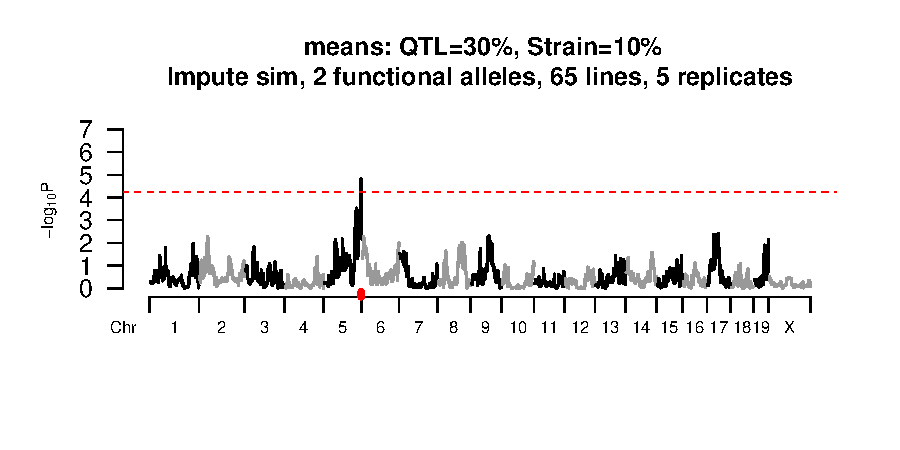
\includegraphics[width=0.75\textwidth, trim={0in 0.9in 0in 0.8in}, clip]{figures/3-sparcc/sample_scan1.pdf}
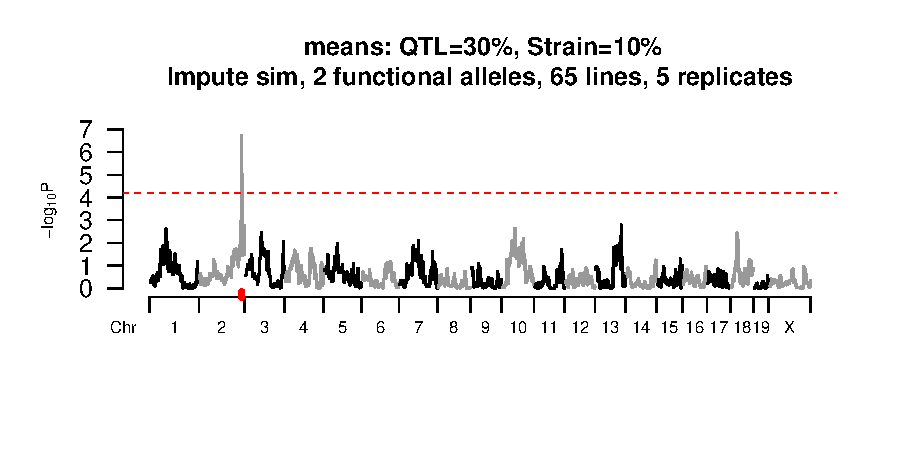
\includegraphics[width=0.75\textwidth, trim={0in 0.9in 0in 0.8in}, clip]{figures/3-sparcc/sample_scan2.pdf}
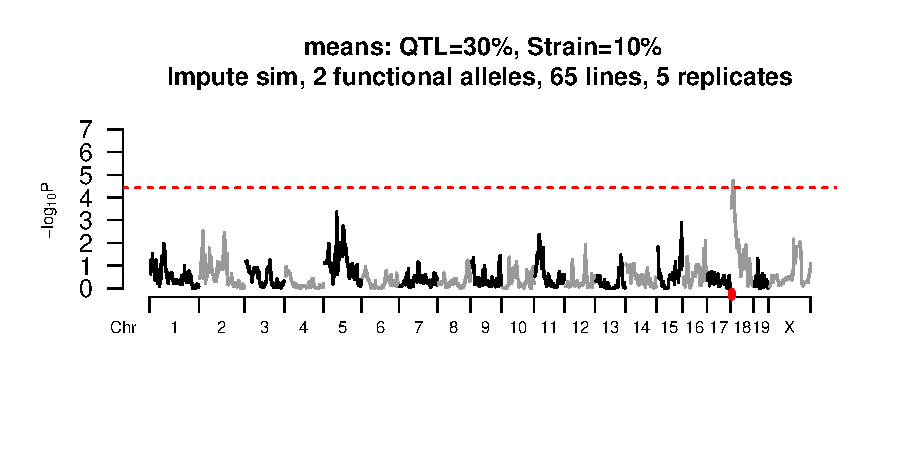
\includegraphics[width=0.75\textwidth, trim={0in 0.9in 0in 0.8in}, clip]{figures/3-sparcc/sample_scan3.pdf}
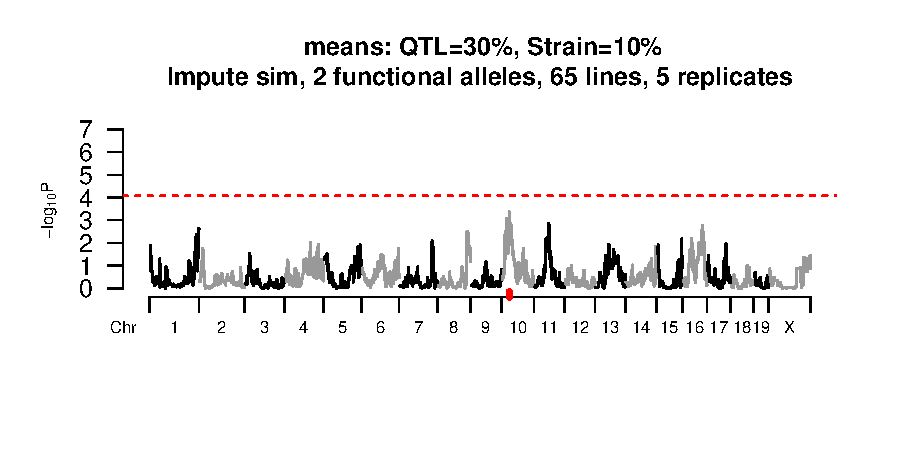
\includegraphics[width=0.75\textwidth, trim={0in 0.9in 0in 0.8in}, clip]{figures/3-sparcc/sample_scan4.pdf}
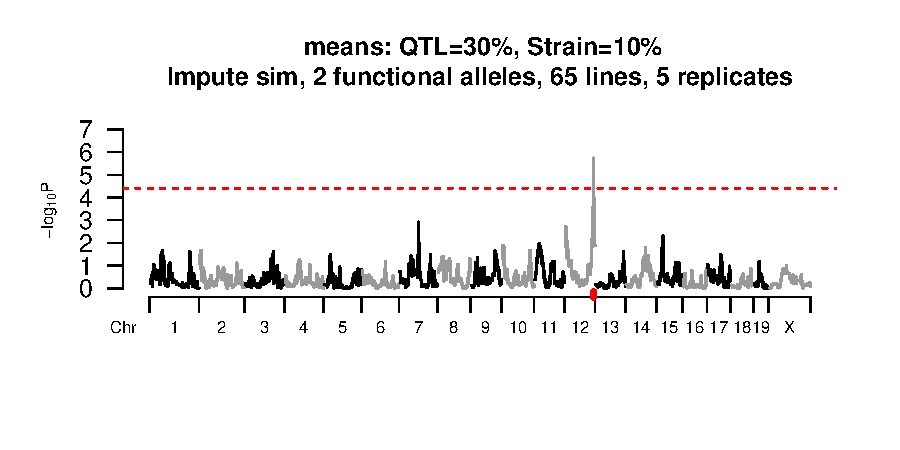
\includegraphics[width=0.75\textwidth, trim={0in 0.7in 0in 0.8in}, clip]{figures/3-sparcc/sample_scan5.pdf}
\caption[Simulated genome scans using SPARCC]{Five simulated genome scans generated by the code provided in the simple SPARCC example. Red dashed lines represent 95\% significance thresholds based on 100 permutation scans. The red tick represents the simulated QTL position. These simulations were based on a specified set of 65 CC strains, five replicate observations of each strain, two functional alleles, 30\% QTL effect, and 10\% strain effect. The QTL is not mapped in the fourth simulation, ranked top to bottom. Actual power calculations should be based upon a greater number of simulations.\label{fig:example_scans}}
\end{figure}

\subsection{Large scale power dynamics}

We have run SPARCC with different combinations of various parameters in order to provide a resource for QTL mapping power in the CC that can be broadly referenced. The specific parameter settings follow:
\begin{itemize}
	\item Number of strains: [\{10-70 by 5\}, 72] 
    \item Number of replicates: [1-10, 20, 50] 
    \item QTL effect size (\%): [0.5, 1, 5, \{10-50 by 10\}]
    \item Number of functional alleles: [2, 3, 8] 
    \item Background strain effect size: [0]
\end{itemize}
CC lines and the position of the QTL were sampled for each simulation, providing estimates of power that are effectively averaged over the CC population. 

\subsubsection{Computing environment}

We performed 1000 simulations (in batches of 100) for each combination of the parameters, resulting in 40,320 individual jobs. These jobs were submitted in parallel to a distributed computing cluster (\url{http://its.unc.edu/rc-services/killdevil-cluster/}). Runtime varied depending on parameter settings and the hardware used, with the longest jobs taking approximately 7 hours to complete.

\subsubsection{Experiment size and power}

We used the results of these simulations to produce power curves that illustrate the relationship between power and the number of strains (\textbf{Figure \ref{fig:powerbystrain}}) or number of replicate observations (\textbf{Figure \ref{fig:powerbyrep}}), for a variety of QTL effect sizes, holding other variables fixed. These power curves provide several insights regarding the power to detect QTL in the CC. In general, we find that studies with small-to-moderate sample sizes are well-powered to detect large effect QTL, but that detecting smaller effect QTL could require many replicates. Detecting QTL with effect sizes $\leq 5\%$ is challenging in the CC, reaching 80\% power to detect an effect size of 5\% when all 72 CC strains are used with greater than 15 replicate observations (\textbf{Figure \ref{fig:powerbyrep}} \textbf{[bottomright]}). Detecting 1\% or 0.5\% QTL would require even higher numbers of strains and replicates. For certain patterns of functional alleles, these curves suggest that mapping QTL with effect sizes $\geq 5\%$ are attainable through the use of more CC strains or more replicate observations.

We also investigated the relationship between power and the total number of mice, particularly focusing on whether additional CC strains or additional replicate observations are more valuable in terms of QTL mapping power. To do this, we calculated the number of mice used in each simulated experiment and interpolated the power at regular grid of values for number of replicates and number of mice. SPARCC generally finds that additional CC strains improve mapping power more than replicate observations, indicated by higher power values for lower numbers of replicate observations while holding number of mice constant in \textbf{Figure \ref{fig:heatmap}}. 

\begin{figure*}
\renewcommand{\familydefault}{\sfdefault}\normalfont
\centering
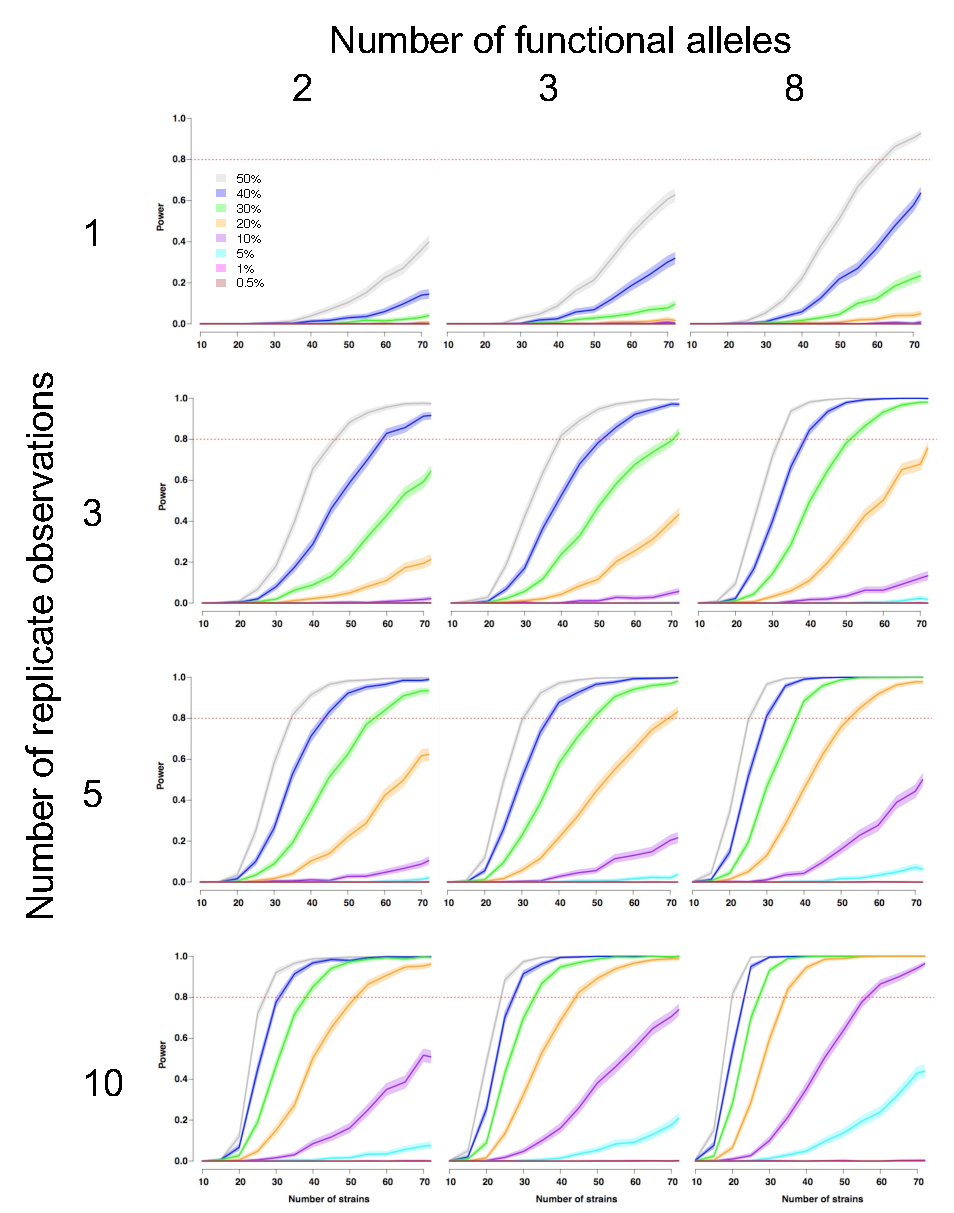
\includegraphics[width=0.8\textwidth, trim={0.1in 0in 0in 0in}, clip]{figures/3-sparcc/power_by_strain_panel.pdf}
\caption[Panel of power curves with respect to number of CC strains]{Power curves based on a thousand simulations per setting with respect to number of CC strains, stratified by number of replicates and the number of functional alleles. The red dashed line emphasizes 80\% power. CC strains and loci were varied in simulations, resulting in powers that average over loci and strain combinations. Confidence intervals were calculated based on Jeffreys interval for a binomial proportion. The columns, left to right, correspond to two functional alleles, three functional alleles, and eight functional alleles. The alternative model fit at each locus is an eight allele model, parameterized with respect to the eight inbred founders. The rows, top to bottom, correspond to a one, three, five, and ten observations of each CC strain. Better power tracks with increased numbers of strains, numbers of replicate observations, and functional alleles. \textbf{Figure \ref{fig:powerbyrep}} has power curves with respect to number of replicate observations rather than number of CC strains. The allelic series for the two and three allele simulations were sampled uniformly, meaning any distribution of functional alleles to founders was given equal probability weight. \label{fig:powerbystrain}}
\end{figure*}

\begin{figure*}
\renewcommand{\familydefault}{\sfdefault}\normalfont
\centering
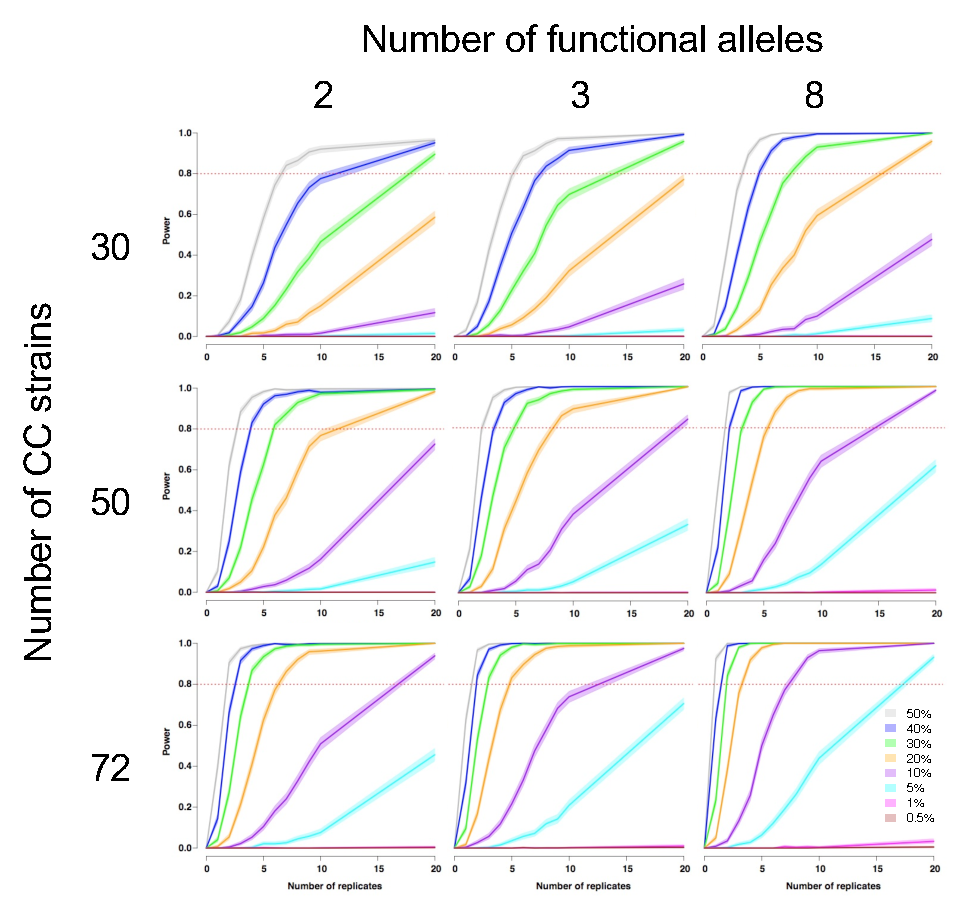
\includegraphics[width=0.9\textwidth, trim={0in 0in 0in 0in}, clip]{figures/3-sparcc/power_by_rep_panel.pdf}
\caption[Panel of power curves with respect to number of replicate observations]{Power curves based on 1000 simulations per setting with respect to number of replicates per CC strain, stratified by number of CC strains and the number of functional alleles. The red dashed line emphasizes 80\% power. CC strains and loci were varied in simulations, resulting in powers that average over loci and strain combinations. Confidence intervals were calculated based on Jeffreys interval for a binomial proportion. The columns, left to right, correspond to two functional alleles, three functional alleles, and eight functional alleles. The alternative model fit at each locus is an eight allele model, parameterized with respect to the eight inbred founders. The rows, top to bottom, are 30, 50, and 72 CC strains. As seen in \textbf{Figure \ref{fig:powerbystrain}}, better power tracks with increased numbers of strains, numbers of replicate observations, and functional alleles. \label{fig:powerbyrep}}
\end{figure*}

\begin{figure}
\renewcommand{\familydefault}{\sfdefault}\normalfont
\centering
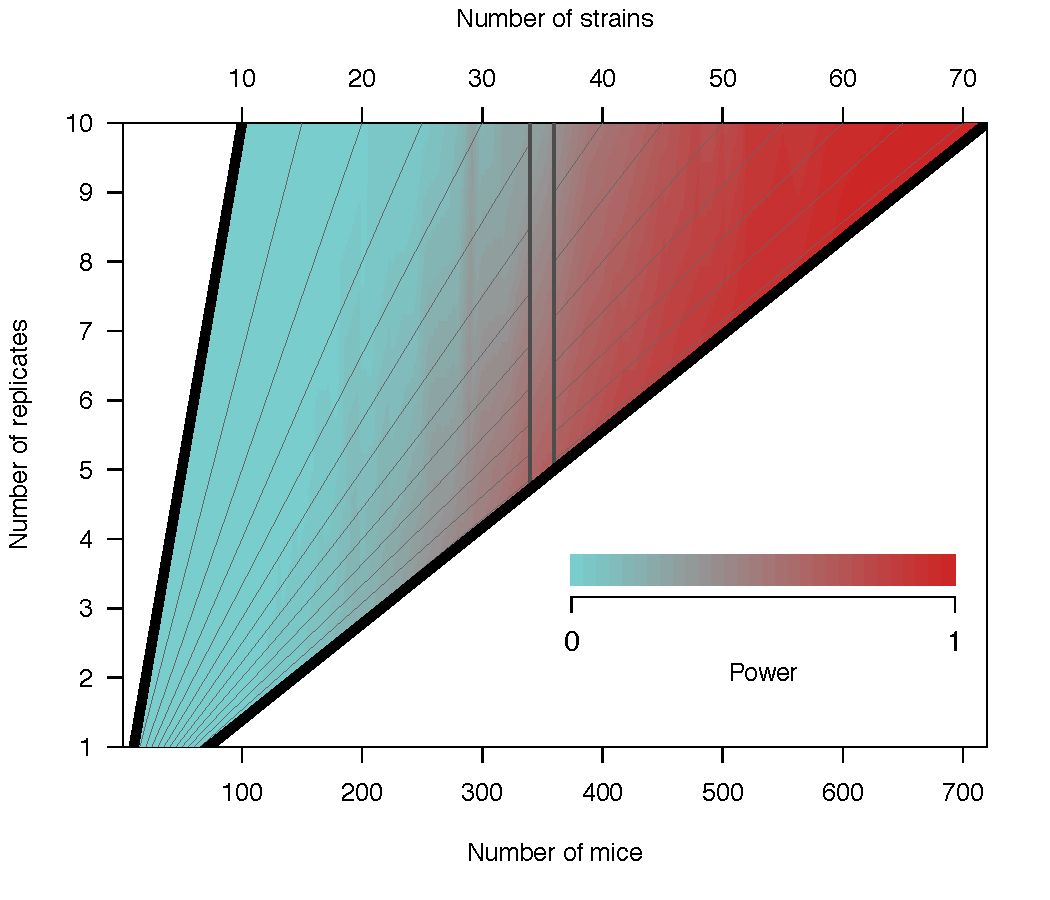
\includegraphics[width=\textwidth, trim={0in 0.1in 0in 0in}, clip]{figures/3-sparcc/power_heatmap_process.pdf}
\caption[Heatmap of power by number of replicate observations and total mice in experiment]{A heatmap of QTL mapping power for number of replicate observations by total number of mice in the experiment. This figure assumes a QTL effect size of 20\%, no background strain effect, and two functional alleles, though varying these parameters should not change the inference. Power was interpolated at regular intervals across a grid of values for number of replicates and number of mice to facilitate plotting, approximating power for numbers of mice that were not directly assessed. Note that some combinations of number of replicate observations and total number of mice are not defined because the CC is limited to 72 strains and we only considered equal numbers of replicates for all strains. The gray diagonal lines represent fixed values of the number of CC strains, ranging from 10 to 70 in intervals of five. Holding the total number of mice fixed, the power reduces as the percentage of the sample that are replicates increases, suggesting that observations of new genomes are more important to QTL mapping power than replicate observations. This is illustrated with a cutout band centered on 350 mice. Power is lower at the top of the band where replicate mice are a relatively higher proportion of the total number of mice. Thus, prioritizing experiments with higher numbers of CC strains rather than higher numbers of replicates is ideal. Increasing the number of replicate observations does benefit QTL mapping power, but not as effectively as additional strains.\label{fig:heatmap}}
\end{figure}

\subsubsection{Allelic series and power}

We emphasize that the overall power depends on the assumed number of functional alleles underlying the QTL. The reasonableness of an assumed number of alleles for a simulation depends on the phenotype. For instance, if the expected causal variant is a single SNP, biallelic QTL are most appropriate, and multiallelic QTL simulations could be overly optimistic. However, a multiallelic QTL can result from local epistatic interactions in the region, which may be more likely with phenotypes closer to the genome, such as gene expression, than physiological phenotypes. 

\subsubsection{Statistical procedure assumes eight alleles} 

Several factors contribute to dependency of power on the number of functional alleles. One component to the reduction in power for QTL with fewer than eight alleles is that the fit alternative model assumes that each founder strain is an allele. For QTL with fewer than eight alleles, some degrees of freedom are being wasted on estimating redundant allele parameters. Power would likely improve for bi-allelic QTL were simpler models used, such as bi-allelic genotypes \citep{Yalcin2005}. The development of alternative mapping approaches that specifically account for the allelic series remains to be adequately addressed, though such approaches will not be trivial and amenable to power calculations. Still, it stands to reason that if the QTL has less than eight functional alleles, a corresponding allelic genome scan would be more powerful than the eight allele model used in SPARCC.

\subsubsection{Observed functional allele frequency imbalance}

Also contributing to reduction in power for QTL with fewer functional alleles than the statistical procedure is the observed allele frequency balance in the data set. While the CC is generally balanced with respect to inheritance from all eight founders across the genome, certain allelic series will result in data that are potentially highly imbalanced in terms of the observed functional alleles. For example, a functional bi-allelic SNP with one allele present in only one of the founder haplotypes will have a minor allele frequency of 12.5\% at a locus that is perfectly balanced in CC. This reduces the variance explained by the QTL effect in the population, and correspondingly, the power to detect that effect.

Taking the allele frequency balance issue to the extreme, though the CC has good average balance with respect to the founder haplotypes, at any given specific loci, one or more alleles may be lost, and thus their functional alleles unobservable. By posing the problem of power estimation in the context of the CC founders and the realized CC strains, the power estimates from SPARCC can reflect the reduction in power to map QTL at loci where potential functional alleles have been lost, which we view as a strength of our approach. SPARCC can produce more optimistic bi-allelic power calculations by fixing the allelic series to be balanced (example: \texttt{M.ID="0,0,0,0,1,1,1,1"}), but in reality, such power calculations are themselves overly-optimistic in assuming that bi-allelic QTL will be balanced across the founder haplotypes. \textbf{Figure \ref{fig:two_alleles}} illustrates the effect that imbalance of the allelic series can have on the power to map QTL in the CC.

\begin{figure}
\renewcommand{\familydefault}{\sfdefault}\normalfont
\centering
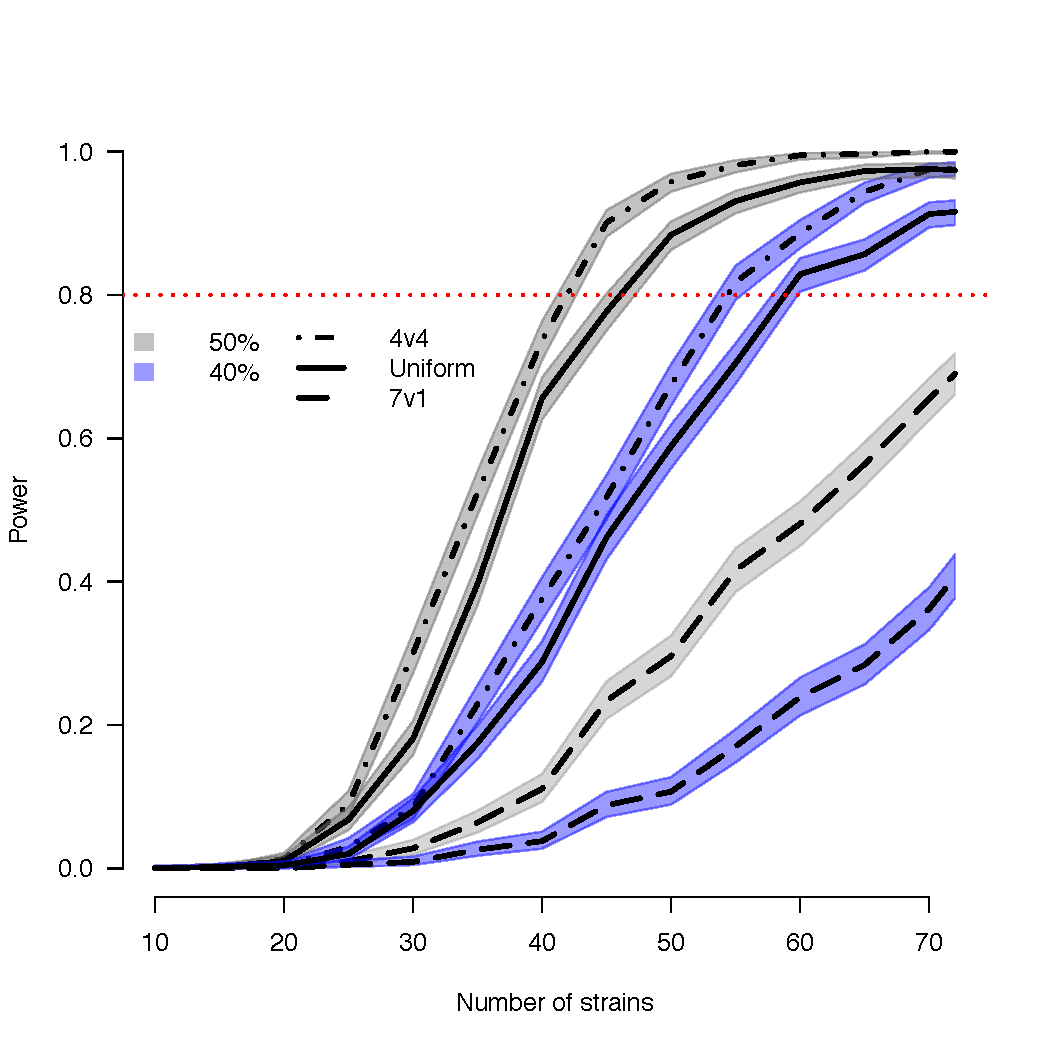
\includegraphics[width=\textwidth, trim={0in 0.2in 0in 0in}, clip]{figures/3-sparcc/two_allele_comparisons_processed.pdf}
\caption[Comparison of power curves for varying allelic series with two functional alleles]{Power curves comparing two QTL effect sizes and four different settings for an allelic series with two functional alleles. These simulations are based on three replicate observations per genome. A balanced representation of the functional alleles, with each allele corresponding to four of the founders (4v4), produces the best power. This is followed closely by uniform sampling of allelic series, in which any bi-allelic allelic series is equally likely (Uniform; the default for SPARCC). Finally, fixing the allelic series at a highly imbalanced setting, one functional allele corresponding to only a single founder (7v1), results in greatly reduced power.\label{fig:two_alleles}}
\end{figure}

\subsection{CC as a mapping population}

SPARCC demonstrates that the CC can be used to effectively map QTL. Though the power calculations in the realized CC are not as optimistic as the simulated expectations of 1000 lines \citep{Valdar2006c}, successful mapping experiments can still be designed, particularly harnessing the ability to have replicate observations. It also bears emphasizing that, aside from mapping, the CC is a powerful tool for new disease models \citep{Rogala2014,Gralinski2015} and as a means of validating results from the DO \citep{Chick2016}.

\subsection{Limitations}

Any analysis of power is subject to the assumptions underlying that analysis. One of the advantages of SPARCC is that its flexibility allows the impact of many of these assumption to be explored. For example, assumptions about how well the strain effect is modeled or the number of independent QTL signals may provide valuable insight into how genetic architecture determines power in the CC. In addition, SPARCC could be used to investigate many related questions, including the power for specific combinations of CC strains or experimental designs, exploring genome-wide false positive rates, or assessing how the power to detect QTL varies depending on genomic position. In terms of future work, the simulation procedure within SPARCC could be expanded to investigate how problems like variance heterogeneity or model mis-specification influence power.

\subsection{Conclusion}

SPARCC is a useful software tool for exploring the power to detect QTL in the CC. This software leverages an efficient model fitting approach in order to explore power in a level of detail that has previously been impractical. This simulation-based approach improves on previous attempts to characterize power in the CC by using the realized CC genomes currently available. We intend that SPARCC will be a useful and flexible tool for researchers designing CC experiments.

\section{Simulation Documentation: Detailed description of \texttt{sim.CC.data()} options}

\subsection{QTL effect}

\begin{itemize}
	\item \texttt{qtl.effect.size}
    \begin{itemize}
    	\item $0 \le \texttt{qtl.effect.size} < 1 - \texttt{strain.effect.size}$ 
    	\item This argument represents $\phi^{2}$, such that $\bbeta \sim \text{N}(\bzero, \bI\phisq)$. 
        \item A specific $\bbeta$ can specified with the \texttt{beta} argument, though it will be scaled to match \texttt{qtl.effect.size}. If \texttt{beta=NULL}, then $\bbeta$ is sampled accordingly.
    \end{itemize}
    
    \item \texttt{num.alleles} (DEFAULT = 8)
    \begin{itemize}
    	\item $2 \le \texttt{num.alleles} \le 8 $
    \end{itemize}
    
    \item \texttt{M.ID}
    \begin{itemize}
    	\item Rather than specifying \texttt{num.alleles} and then sampling $\bM$, these can be fixed with the \texttt{M.ID} argument.
        \item Expects strings of the form \texttt{"A,B,C,D,E,F,G,H"}, with each letter corresponding to a founder strain, taking an integer value 0-7, representing functional alleles.
        \item Example: \texttt{M.ID="0,0,0,0,1,1,1,1"} represents a biallelic causal variant, in which the first four strains have one allele, and the last four having the other.
    \end{itemize}

    \item \texttt{CC.lines} (DEFAULT = NULL)
    \begin{itemize}
    	\item This argument allows the user to provide a vector of CC line IDs on which to base the power calculation. The CC genomes, along with \texttt{locus}, will determine $\bD$ in Eq \ref{eq:sdp}. 
        \item If \texttt{CC.lines = NULL}, then SPARCC will sample \texttt{num.lines} from all available lines. 
        \begin{itemize}
        	\item \texttt{vary.lines} (DEFAULT = TRUE)
            \begin{itemize}
        		\item If \texttt{vary.lines = TRUE}, the set of lines for each simulation will be sampled and vary.
                \item If \texttt{vary.lines = FALSE}, the set of lines will be sampled once, and used for each simulated outcome.
            \end{itemize}
        \end{itemize}
    \end{itemize}
    
    \item \texttt{locus} (DEFAULT = NULL)
    \begin{itemize}
    	\item This argument allows the user to specify a specific locus for the simulated QTL, in effect determining the haplotype dosage matrix $\bD$. 
        \item If the argument is left empty, SPARCC will sample loci uniformly from the CC genomes, thus providing power estimates averaged over genomic positions.
    \end{itemize}
    
    \item \texttt{impute} (DEFAULT = TRUE)
    \begin{itemize}
    	\item If \texttt{impute=TRUE}, then $\bD$ in Eq \ref{eq:sdp} is sampled from the probabilistically reconstructed diplotypes at the QTL
        \begin{equation}
        	\bD_{i} \sim \text{Cat}(\bP_{i})
        \end{equation}
        where $\text{Cat}(.)$ is a categorical distribution and $\bP$ is a matrix of diplotype probabilities for the CC genomes at the QTL.
        \item If \texttt{impute=FALSE}, then $\bD = \bP$ in the simulation procedure.
    \end{itemize}
    \item \texttt{scale.qtl.mode} (DEFAULT = "B")
    \begin{itemize}
    	\item If \texttt{scale.qtl.mode="B"}, $\text{var}(2\bbeta)$ is scaled to \texttt{qtl.effect.size}, setting the QTL effect size with respect to a theoretical population that is balanced with respect to functional alleles, from which the CC mapping population developed. 
        \item If \texttt{scale.qtl.mode="MB"}, $\text{var}(2\bM\bbeta)$ is scaled to \texttt{qtl.effect.size}, setting the QTL effect size to a theoretical natural-like population with a specific allelic series.
	\item If \texttt{scale.qtl.mode="DAMB"}, $\text{var}(\bD\bA\bM\bbeta)$ is scaled to \texttt{qtl.effect.size}, setting the QTL effect size to a specific set of CC strains and allele series.
    \item If \texttt{scale.qtl.mode="ZDAMB"}, $\text{var}(\bZ\bD\bA\bM\bbeta)$ is scaled to \texttt{qtl.effect.size}, setting the QTL effect size with respect to the specific set of CC strain, allelic series, and number of replicate observations.
    \item If \texttt{scale.qtl.mode="none"}, $\bbeta$ is not scaled, allowing the user to specify an effect vector without it being scaled.
    \end{itemize}
\end{itemize}

\subsection{Strain effect}

\begin{itemize}
	\item \texttt{strain.effect.size}
    \begin{itemize}
    	\item $0 \le \texttt{strain.effect.size} \le 1 - \texttt{qtl.effect.size}$
    	\item This argument specifies $\tausq$, such that $\bdelta \sim \text{N}(\bzero, \bI\tausq)$.
    \end{itemize}
\end{itemize}
The actual sampled strain effect are scaled in the same manner as the QTL effect, which is specified with \texttt{scale.by.var}.

\subsection{Additional options}

\begin{itemize}
	\item \texttt{num.sim}
    \begin{itemize}
    	\item This argument specifies SPARCC to simulate $s$ samples of $\by$ from Eq \ref{eq:general_sim}.
    \end{itemize}
    \item \texttt{num.replicates}
    \begin{itemize}
    	\item This argument allows the user to set the number $r$ of replicate observations of each CC line. The reproducibility of CC genomes is an important feature, allowing noise variation to be reduced.
        \item SPARCC currently requires all CC lines to have the same number of replicates.    
    \end{itemize}
\end{itemize}


